\chapter{応用例}
\label{chap:usage}

本章では、HypAR Touchによって実現可能な応用例について述べる。

\newpage


\section{駅など公共施設での案内}
駅や空港などの比較的大規模な公共施設内ではGPSによる案内が利用できない場合が多く、2次元の地図を提示するか矢印などによる案内表示を行うのが一般的である。
しかしながら両者にはそれぞれ案内システムとして問題が存在する。
2次元の地図は内部構造が複雑な屋内を表現することが難しく、地下鉄ホームなどの複雑な地形の案内に不向きである。
また設置できる場所に限りがあり、必要な時に参照できないことがある。
矢印などによる案内表示の場合、記述できる情報に限りがあり、必ずしも自分の目的地に沿う案内があるとは限らないという問題点がある。

これらの従来の案内システムと比べ、本システムではARで目的地を直接提示(図:\ref{fig:ar_navigation_shonandai})するため地図の苦手な人への案内や複雑な構造の施設の案内において有用である。
またNFCタグは一枚あたり十数円と安価で、サイズも小さいため設置場所やコストに困るケースは少ないといえる。
さらにNFCタグに紐付いた情報により表示するAR情報のあるScrapboxプロジェクトやハイパーリンクによるフィルターを指定できる。
そのため駅の出口だけを案内したり(図:\ref{fig:ar_navigation_exit})広告として特定店舗だけを案内したり(図:\ref{fig:ar_navigation_ad})といった特定の用途に特化した案内をすることも可能である。

\begin{figure}[h]
  \begin{minipage}{0.5\hsize}
    \centering
    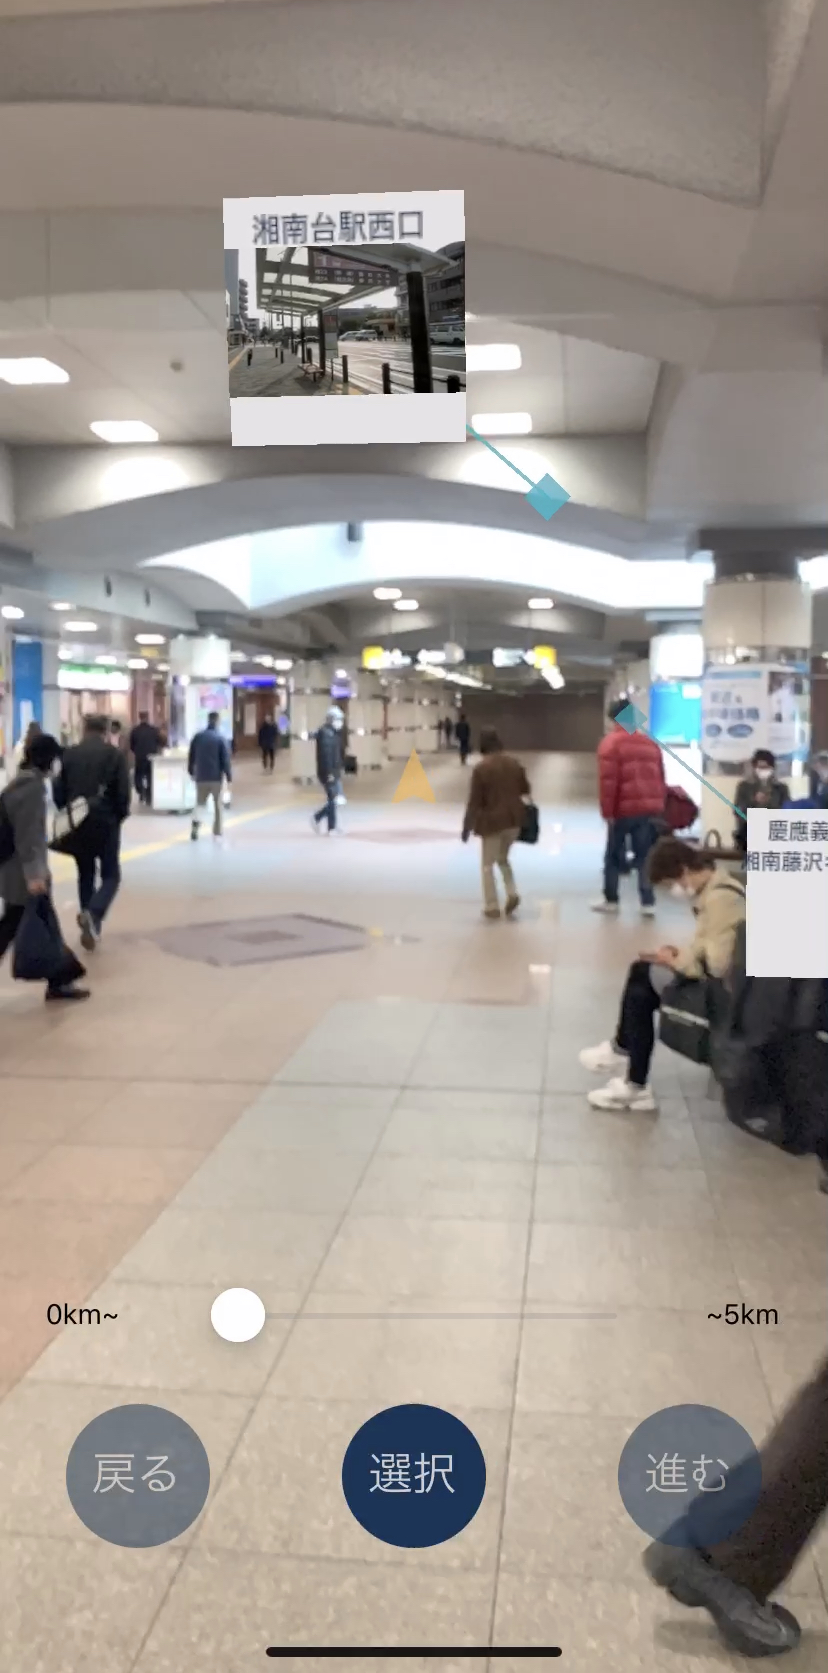
\includegraphics[width=60mm]{images/ar_navigation_shonandai.jpg}
    \caption{案内の様子} \label{fig:ar_navigation_shonandai}
  \end{minipage}
  \begin{minipage}{0.5\hsize}
    \centering
    
\includegraphics[width=60mm]{images/wip2.jpg}
    \caption{出口だけの案内} \label{fig:ar_navigation_exit}
  \end{minipage}
\end{figure}

\begin{figure}[h]
  \centering
  
\includegraphics[width=60mm]{images/wip2.png}
  \caption{リンクを利用したルートの表記例} \label{fig:ar_navigation_ad}
\end{figure}

\section{近隣施設の探索・推薦}

本システムの大きな特徴としてWikiを利用することにより情報を階層化せずに関連情報を参照できる点が挙げられる。
その結果以下のような探索がAR上で行える
\begin{itemize}
  \item 近隣施設の情報にあるリンクから関連情報を参照する
  \item 関連情報から興味のあるジャンルの店舗を発見する
  \item 履歴機能を使いながらほかの情報を比較する
\end{itemize}
上記のような能動的探索行為は目的地への案内のみを目的としている既存のアプリケーションでは体験できないものである。

例えば神保町で本システムを利用した場合、ウィンタースポーツ用品店を選択すれば、「スノーボード」「スキー」といったいったリンクが出現する(図\ref{fig:ar_navigation_jibotyo_ski})。
ウィンタースポーツ用品店をめぐりたい場合はこれらのリンクを選択することでウィンタースポーツに関連する施設の情報を見ることができる。

またその後食事をを取りたくなった場合、興味のある飲食店を選択することで「ラーメン」「カレー」等のリンクが出現し自身の食べたいものを絞り込み(図\ref{fig:ar_navigation_jibotyo_lunch})、他の情報と比較しながら探索できる。

このように本システムは様々な施設の情報が混在していてもリンクを選択していくことで自分の求める情報を探索でき、既存のARナビゲーションアプリケーションにない魅了を持った非常に拡張性も高いシステムであると言える。


\begin{figure}[h]
  \begin{minipage}{0.5\hsize}
    \centering
    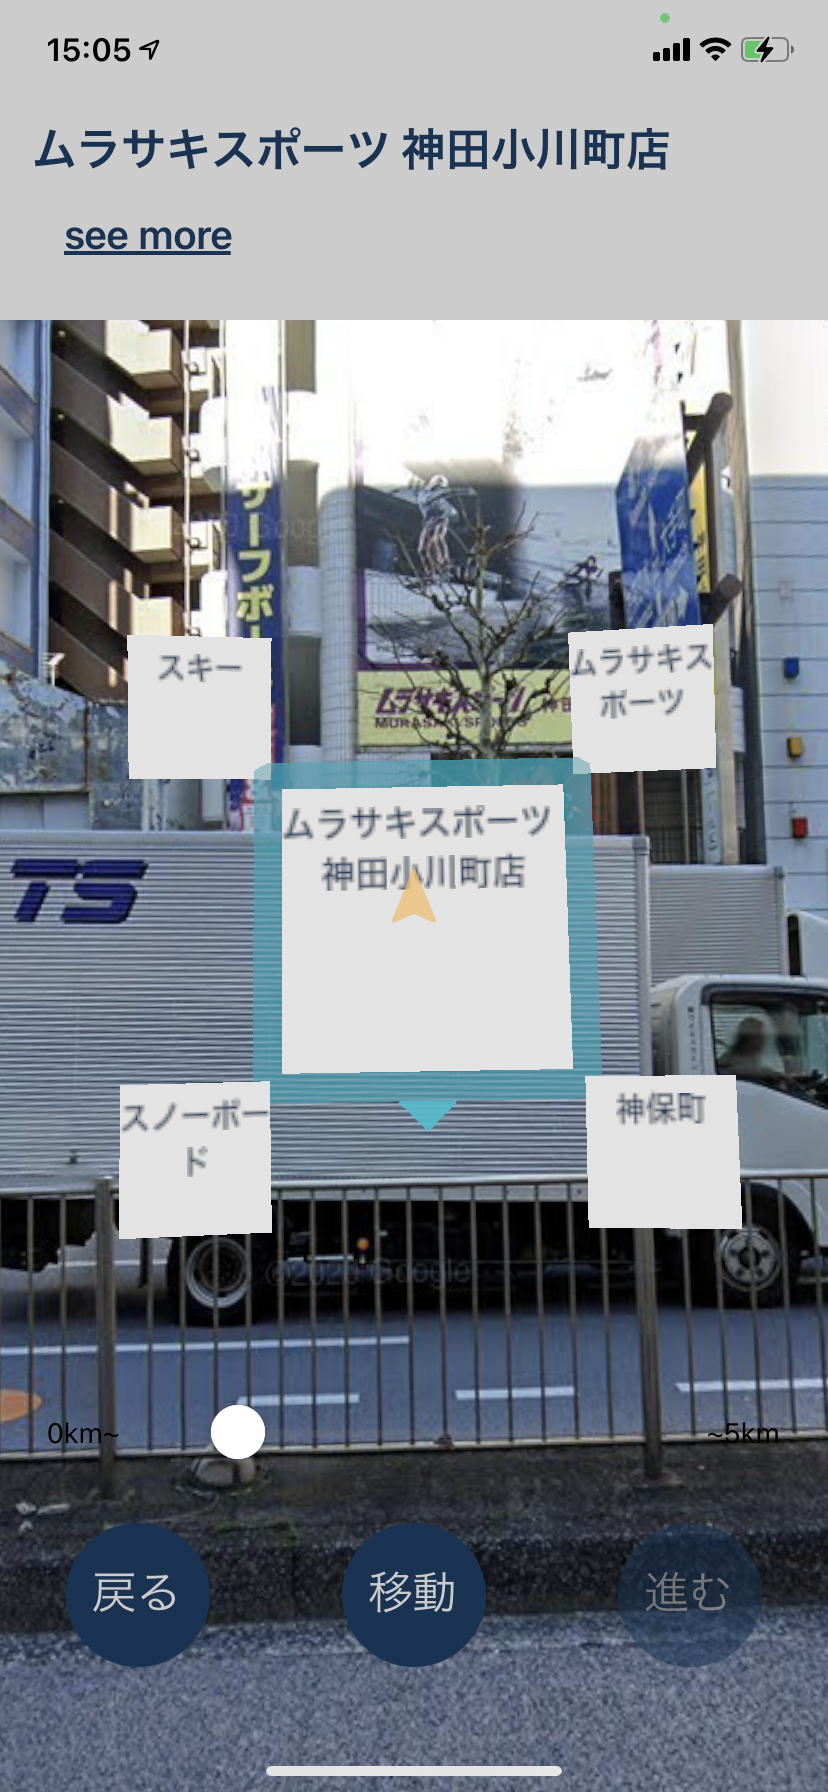
\includegraphics[width=60mm]{images/ar_navigation_jibotyo_ski.png}
    \caption{スキーのリンクを選択した時} \label{fig:ar_navigation_jibotyo_ski}
  \end{minipage}
  \begin{minipage}{0.5\hsize}
    \centering
    
\includegraphics[width=60mm]{images/wip2.jpg}
    \caption{飲食店を選択した時} \label{fig:ar_navigation_jibotyo_lunch}
  \end{minipage}
\end{figure}


\section{学習教材としての利用}
wikiはwikipediaに代表されるように膨大な史実や地理情報を整理し、記録するのに適したメディアであると言える。
本システムではwikiの各ページに位置情報を記載するだけでページの情報をARでの表示できるため、地理情報を含む歴史や地理の教材として利用することが可能である。

例として京都など史跡が多い地域でのフィールドワークに利用することなどが考えられる。
学習者は各地にあるタグに触れるだけで周辺にある史跡の情報見ることができるだけでなく、選択した史跡の関連情報から他の史跡の情報や位置をARで見ることができる。
これにより自身の興味や学習対象に関連する史跡を効率よく回り、自身の知らない史跡を知る事ができる。

さらに本システムでは第3章で述べた通り現在地からのAR表示だけでなく選択されたAR情報の場所に視点を移動する事が可能である。
この機能によって実際の場所にいなくとも関連情報を元に視点を切り替えながら史跡を見ることが可能である。

% TODO:移動機能での強み


\section{リンクを利用した柔軟な参照}
\label{link_enum_notation}
本システムでは位置情報を記載したScrapboxページを作成することでAR情報を登録することができるが、それに加えて登録されたAR情報のリンクを利用した新しいページを作ることも可能である。

例えば渋谷からSFCのキャンパスまでの経路を記述したい場合は図のように登録した場所のリンクを列挙すること表現することができる。
Scrapbox上では単にリンクを並べただけだが、HypAR Touchアプリ側では図(準備中)のように通るべきポイントがARで表示される。

% TODO:博物館的な案内もかける

このような書き方はユーザによって簡単に行えるだけでなく、表記の揺れにも強いという利点を持っている。

\begin{figure}[h]
  \centering
  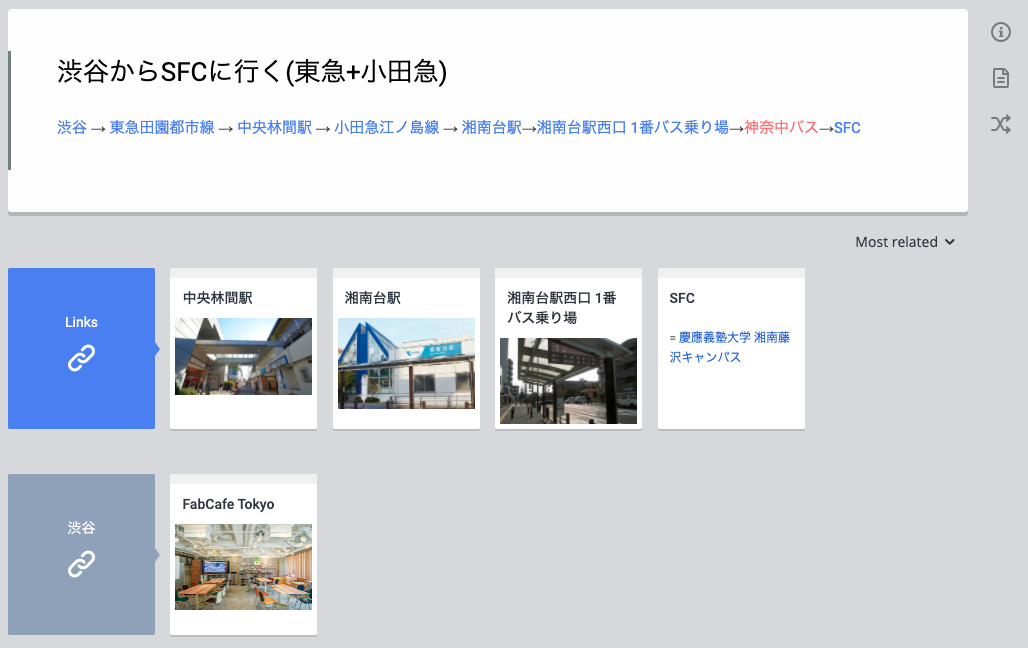
\includegraphics[width=150mm]{images/route_scrapbox.png}
  \caption{リンクを利用したルートの表記例} \label{fig:route_scrapbox}
\end{figure}


\section{まとめ}
本章では、本システムによって実現可能な、NFCタグによるインタラクションとリンクによる関連情報の表示機能を活かした利用例について述べた。
タッチというわかりやすいインタラクション、Wikiの持つ拡張性などから、本章で述べた利用例に限らず様々な応用が可能であると考えられる。